    \documentclass[12pt]{article}

        \usepackage[dvipsnames,svgnames,x11names]{xcolor}
        \usepackage{graphicx}
        \usepackage{tikz}
        \usepackage{amsmath}
        \usepackage[fleqn,tbtags]{mathtools}
        \usepackage{physics}
        \usepackage{array}
        \usepackage{geometry}
        \usepackage{hyperref}
        \usepackage{multirow}
        \usepackage{makecell}
        \usepackage{supertabular}
        \usepackage{longtable}
        
        
        \geometry{
            top=1in,
            left=1in,
            right=1in,
            bottom=1in
        }
        % Definir el ancho total disponible
        \newlength{\totalwidth}
        \setlength{\totalwidth}{\textwidth}

        % Calcular anchos de columna para la tabla principal
        \newlength{\firstcolwidth}
        \setlength{\firstcolwidth}{0.25\totalwidth}
        \newlength{\othercolwidth}
        \setlength{\othercolwidth}{0.25\totalwidth}

        % Comandos básicos
        \newcommand{\ans}[1]{\textbf{\color{black} #1}}
        \renewcommand{\vec}[1]{\boldsymbol{#1}}
        \newcommand{\unitvec}[1]{\boldsymbol{\hat{#1}}}

        % Tipos de columna personalizados
        \newcolumntype{Y}{>{\centering\arraybackslash}p{\othercolwidth}}
        \newcolumntype{Z}{>{\centering\arraybackslash}p{\firstcolwidth}}

    \begin{document}
        \title{Comparación de los métodos de selección}
        \author{
            Alberto Valentín Velásquez Santos \\
            Harold Mondragon Tavara and \\
            Max Houston Ramirez Martel \\
            Rodolfo Morocho Caballero \\
        }
            
        % \author{The Bankers}
        \date{Noviembre 2024}
        \maketitle
        \renewcommand{\contentsname}{Índice}  % Cambiar título
        \tableofcontents
        \setcounter{tocdepth}{3}

        \section{Implementación}
        \begin{itemize}
            \item \textbf{Experimento 1:} 
            \href{https://colab.research.google.com/drive/1S57At2Zv09vkb5BnqWQWhOzGMQPR1V_f?usp=sharing}{\textcolor{blue}{Código fuente del experimento en Colab}}
            
            \item \textbf{Experimento 2:} 
            \href{https://colab.research.google.com/drive/1DwuVdfqbHCSGKmwRBW1Oex84BFJMk7Mc?usp=sharing}{\textcolor{blue}{Código fuente del experimento en Colab}}
        \end{itemize}
        \section{Resultados}
            \subsection[Experimento 1]{Experimento 1: Comparación de métodos de selección}
                Para un mismo conjunto de 100 ciudades, implementar y comparar la solución obtenida usando los métodos de selección: Roulette wheel selection Rank-based selection, Fitness scaling y Tournament selection.
                \subsubsection[Roulette Wheel Selection]{Roulette Wheel Selection}
                    Consiste en que la probabilidad de ser elegido es proporcional al fitness y cada elemento ocupa un segmento para ser elegido.
                
                \subsubsection[Rank Based Selection]{Rank Based Selection}
                    La probabilidad está en función al rango o posición de los elementos de una población, cada elemento se ordena según el fitness.
                
                \subsubsection[Fitness Scaling Selection]{Fitness Scaling Selection}
                    El fitness de cada elemento se realiza un escaldo lineal o adaptativo antes del proceso de selección.

                \subsubsection[Tournament Selection]{Tournament Selection}
                    Este método consiste en elegir de forma aleatoria elementos de una población quedando solo con el óptimo.
                \vspace{3mm}
                
                \begin{longtable}{|>{\centering\arraybackslash}p{0.15\textwidth}|*{4}{>{\centering\arraybackslash}p{0.2\textwidth}|}}
                    \caption{Resultados de los métodos de selección} \label{tab:selection_results} \\
                    \hline
                    \multicolumn{1}{|c|}{\multirow{2}{*}{\rule{0pt}{4ex}Generación}} & \multicolumn{4}{c|}{Fitness} \\[2ex]
                    \cline{2-5}
                    & \rule{0pt}{3ex}\makecell{Roulette\\Wheel\\Selection} & \makecell{Rank-Based\\Selection} & \makecell{Fitness\\Scaling\\Selection} & \makecell{Tournament\\Selection} \\[1.5ex]
                    \hline
                    \endfirsthead
                    
                    \multicolumn{5}{c}{\tablename\ \thetable{} -- Continuación} \\
                    \hline
                    \multicolumn{1}{|c|}{\multirow{2}{*}{\rule{0pt}{4ex}Generación}} & \multicolumn{4}{c|}{Fitness} \\[2ex]
                    \cline{2-5}
                    & \rule{0pt}{3ex}\makecell{Roulette\\Wheel\\Selection} & \makecell{Rank-Based\\Selection} & \makecell{Fitness\\Scaling\\Selection} & \makecell{Tournament\\Selection} \\[1.5ex]
                    \hline
                    \endhead
                    \rule{0pt}{4ex}0 & 46.0405753 & 45.372529 & 47.1906354 & 45.5480999 \\[1ex]
                    \hline
                    \rule{0pt}{4ex}200 & 21.7275399 & 45.372529 & 27.3317811 & 16.2008103 \\[1ex]
                    \hline
                    \rule{0pt}{4ex}400 & 17.4071704 & 45.372529 & 23.3323755 & 12.0895081 \\[1ex]
                    \hline
                    \rule{0pt}{4ex}600 & 14.2522011 & 44.1501087 & 19.9919763 & 10.372674 \\[1ex]
                    \hline
                    \rule{0pt}{4ex}800 & 12.8809428 & 43.9863321 & 18.7416694 & 9.90466136 \\[1ex]
                    \hline
                    \rule{0pt}{4ex}1000 & 12.6590962 & 42.7031294 & 16.6458018 & 9.90466136 \\[1ex]
                    \hline
                    \rule{0pt}{4ex}1200 & 12.532009 & 42.7031294 & 15.43604 & 9.8294855 \\[1ex]
                    \hline
                    \rule{0pt}{4ex}1400 & 12.4233396 & 42.7031294 & 14.9056858 & 9.74728195 \\[1ex]
                    \hline
                    \rule{0pt}{4ex}1600 & 12.1921104 & 42.7031294 & 14.3798882 & 9.59585609 \\[1ex]
                    \hline
                    \rule{0pt}{4ex}1800 & 11.9874773 & 42.7031294 & 13.6739941 & 9.12644879 \\[1ex]
                    \hline
                    \rule{0pt}{4ex}2000 & 11.1098868 & 42.3230657 & 12.6565647 & 9.11431122 \\[1ex]
                    \hline
                    \rule{0pt}{4ex}2200 & 10.7993498 & 41.8715207 & 11.9694388 & 8.93188524 \\[1ex]
                    \hline
                    \rule{0pt}{4ex}2400 & 10.5744095 & 41.5596853 & 11.814441 & 8.92229561 \\[1ex]
                    \hline
                    \rule{0pt}{4ex}2600 & 10.5310081 & 40.4733506 & 11.8080908 & 8.92229561 \\[1ex]
                    \hline
                    \rule{0pt}{4ex}2800 & 10.4720815 & 40.4733506 & 11.8080908 & 8.8645615 \\[1ex]
                    \hline
                \end{longtable}
                
                \begin{figure}[!b]
                    \centering
                    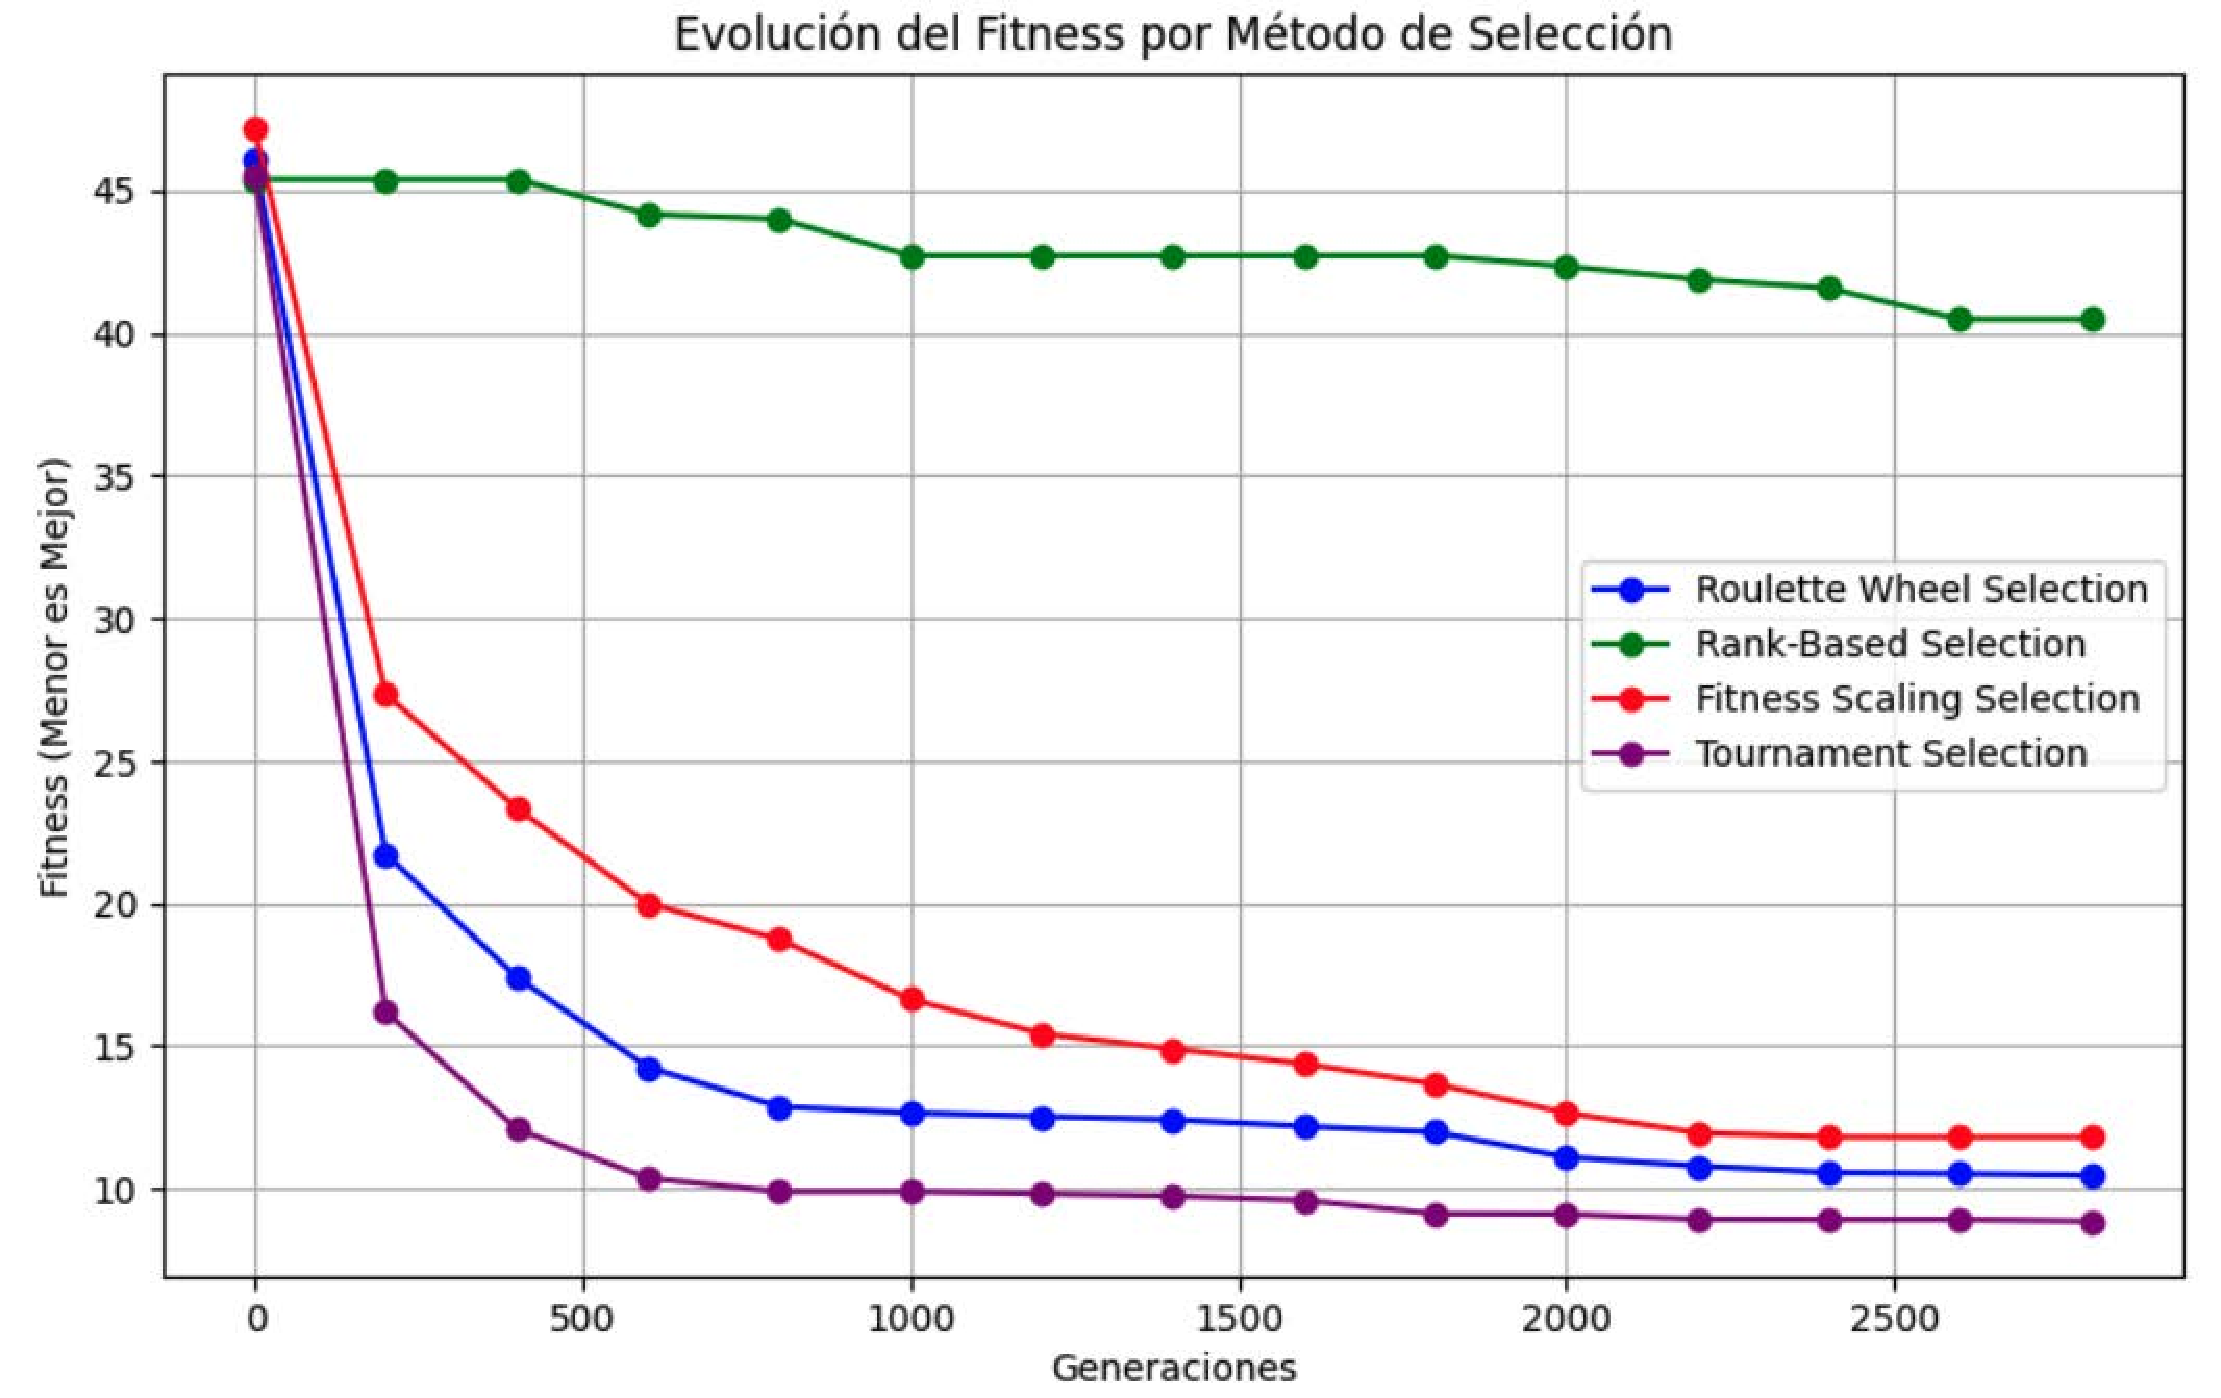
\includegraphics[width=\textwidth]{figure/experimento1_grafico.pdf}
                    \caption{Evolución del Fitness por Método de Selección}
                    \label{fig:selection_methods}
                \end{figure}
            
            \subsection[Experimento 2]{Experimento 2: Comparación de métodos de inicialización de población}
                Para un mismo conjunto de 100 ciudades, implementar y comparar la solución obtenida usando los métodos inicialización de población: random, heuristic y hybrid initialization.
            \subsubsection[Random]{Random}
                La inicialización aleatoria es sencilla de implementar y promueve la diversidad al cubrir una amplia porción del espacio de búsqueda, lo que mejora la capacidad de exploración del algoritmo. Sin embargo, también puede generar soluciones inviables o de baja calidad, desperdiciando recursos computacionales y ralentizando la convergencia.
            \subsubsection[Heuristic]{Heuristic}
                La inicialización heurística emplea técnicas heurísticas para construir soluciones viables y de alta calidad, a las que luego añade perturbaciones aleatorias para mantener la diversidad. Este enfoque puede acelerar la convergencia, pero existe el riesgo de reducir la diversidad, lo que podría resultar en una convergencia prematura o en óptimos locales.
            \subsubsection[Hybrid Initialization]{Hybrid Initialization}
                La inicialización híbrida combina dos enfoques: una parte de las soluciones se genera de manera aleatoria, mientras que otra parte se genera mediante métodos heurísticos. Posteriormente, ambos conjuntos de soluciones se combinan para formar la población inicial.
                
                
                \begin{longtable}{|>{\centering\arraybackslash}p{0.15\textwidth}|*{3}{>{\centering\arraybackslash}p{0.2\textwidth}|}}
                    \caption{Resultados de los métodos de inicialización} \label{tab:initialization_results} \\
                    \hline
                    \multicolumn{1}{|c|}{\multirow{2}{*}{\rule{0pt}{4ex}Generación}} & \multicolumn{3}{c|}{Fitness} \\[2ex]
                    \cline{2-4}
                    & \rule{0pt}{3ex}\makecell{Random} & \makecell{Heuristic} & \makecell{Hybrid} \\[1.5ex]
                    \hline
                    \endfirsthead
                    
                    \multicolumn{4}{c}{\tablename\ \thetable{} -- Continuación} \\
                    \hline
                    \multicolumn{1}{|c|}{\multirow{2}{*}{\rule{0pt}{4ex}Generación}} & \multicolumn{3}{c|}{Fitness} \\[2ex]
                    \cline{2-4}
                    & \rule{0pt}{3ex}\makecell{Random} & \makecell{Heuristic} & \makecell{Hybrid} \\[1.5ex]
                    \hline
                    \endhead
                    \rule{0pt}{4ex}0 & 42.74458451 & 8.37021557 & 8.37021557 \\[1ex]
                    \hline
                    \rule{0pt}{4ex}200 & 21.04099329 & 8.20669462 & 8.15644116 \\[1ex]
                    \hline
                    \rule{0pt}{4ex}400 & 21.04099329 & 8.20669462 & 8.15644116 \\[1ex]
                    \hline
                    \rule{0pt}{4ex}600 & 15.42234724 & 8.20669462 & 8.15644116 \\[1ex]
                    \hline
                    \rule{0pt}{4ex}800 & 14.43601409 & 8.20243297 & 8.15644116 \\[1ex]
                    \hline
                    \rule{0pt}{4ex}1000 & 13.54744598 & 8.14470131 & 8.15644116 \\[1ex]
                    \hline
                    \rule{0pt}{4ex}1200 & 13.15987654 & 8.14470131 & 8.15644116 \\[1ex]
                    \hline
                    \rule{0pt}{4ex}1400 & 12.50920738 & 8.10896400 & 8.15644116 \\[1ex]
                    \hline
                    \rule{0pt}{3ex}1600 & 11.73635878 & 8.10260702 & 8.13414460 \\[1ex]
                    \hline
                    \rule{0pt}{3ex}1800 & 10.83783294 & 8.10260702 & 8.13414460 \\[1ex]
                    \hline
                    \rule{0pt}{4ex}2000 & 10.83783294 & 8.10260702 & 8.13414460 \\[1ex]
                    \hline
                    \rule{0pt}{4ex}2200 & 10.81697066 & 8.10260702 & 8.13414460 \\[1ex]
                    \hline
                    \rule{0pt}{4ex}2400 & 10.78378629 & 8.10260702 & 8.13414460 \\[1ex]
                    \hline
                    \rule{0pt}{4ex}2600 & 10.65365191 & 8.10260702 & 8.13414460 \\[1ex]
                    \hline
                    \rule{0pt}{4ex}2800 & 10.56273547 & 8.10260702 & 8.13414460 \\[1ex]
                    \hline
                \end{longtable}
                \begin{figure}[hbt]
                    \centering
                    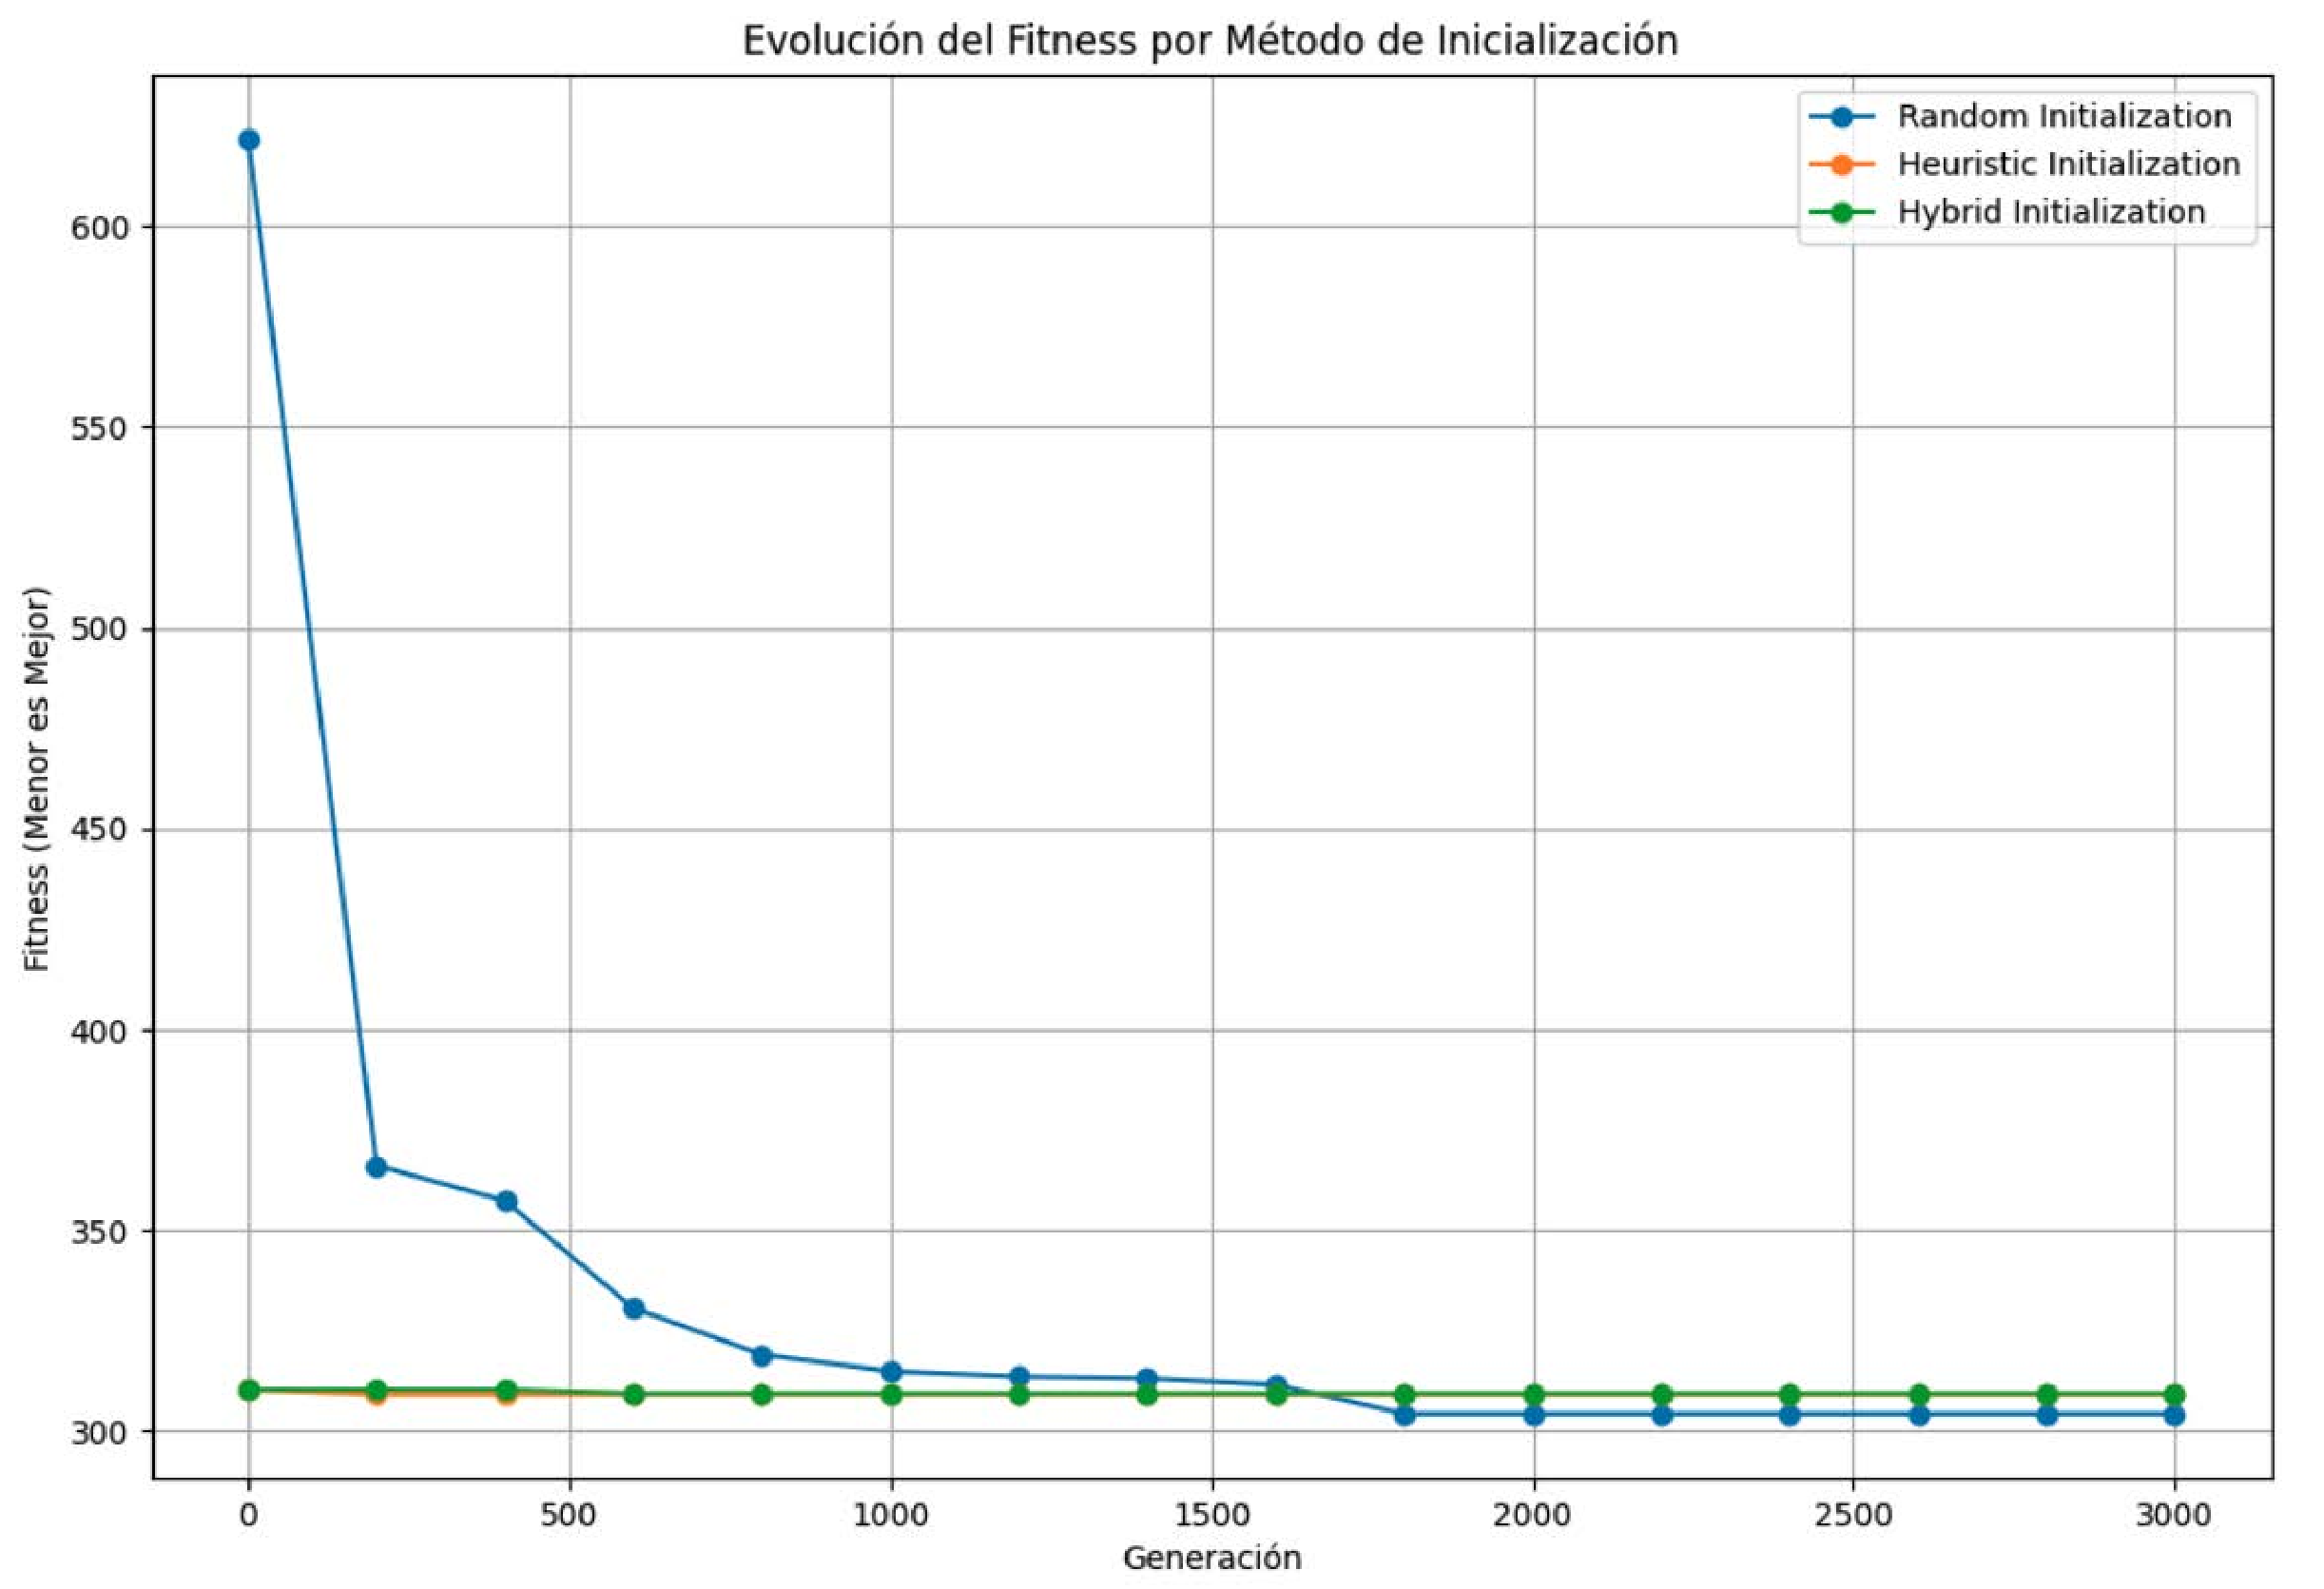
\includegraphics[width=\textwidth]{figure/experimento2_grafico.pdf}
                    \caption{Evolución del Fitness por Método de Inicialización}
                    \label{fig:initialization_methods}
                \end{figure}
        \section{Discusión}
            A partir de los resultados experimentales obtenidos, es importante analizar el comportamiento y las implicaciones de los diferentes métodos evaluados para el problema del TSP con 100 ciudades.
            En el primer experimento, que examina los métodos de selección, se observa una clara diferencia en la eficiencia de cada estrategia. \textit{Tournament Selection} demuestra una superioridad significativa, logrando converger a un fitness de 8.86. Este resultado sugiere que la presión selectiva ejercida por este método es más efectiva para mantener un balance adecuado entre exploración y explotación del espacio de búsqueda. Por otro lado, \textit{Roulette Wheel Selection}, aunque menos efectivo, muestra una capacidad de mejora constante, alcanzando un fitness de 10.47. Es notable que \textit{Rank-Based Selection} presenta limitaciones considerables, evidenciadas por su estancamiento en 40.47, lo que podría indicar una pérdida prematura de diversidad en la población.
            Respecto al segundo experimento sobre métodos de inicialización, los resultados revelan aspectos interesantes sobre la importancia de la población inicial. La inicialización \textit{Heuristic} y \textit{Hybrid} alcanzan rápidamente valores óptimos (8.10 y 8.13 respectivamente), lo que sugiere que incorporar conocimiento específico del dominio en la fase inicial acelera significativamente la convergencia. Sin embargo, es destacable que la inicialización \textit{Random}, a pesar de partir de un fitness considerablemente peor (42.74), logra una mejora sustancial hasta 10.56. Este comportamiento podría indicar que, aunque menos eficiente en términos de velocidad de convergencia, la inicialización aleatoria mantiene una diversidad que permite una exploración más amplia del espacio de soluciones.
            La comparación entre ambos experimentos sugiere que la elección del método de inicialización tiene un impacto más significativo en el rendimiento general del algoritmo que el método de selección. Esto se evidencia en la menor variabilidad de los resultados finales entre los métodos de selección en comparación con los métodos de inicialización. Además, la combinación de una inicialización informada (\textit{Heuristic} o \textit{Hybrid}) con \textit{Tournament Selection} podría representar la estrategia más robusta para abordar este problema específico del TSP.
            Es importante señalar que estos resultados podrían estar influenciados por las características específicas del problema de 100 ciudades y los hiperparámetros seleccionados. La escalabilidad de estas conclusiones a problemas de diferentes dimensiones o con distintas características topológicas requeriría investigación adicional. 

    \end{document}